\documentclass[12pt,a4paper]{article}
\usepackage[utf8x]{inputenc}
\usepackage{ucs}
\usepackage[spanish]{babel}
\usepackage{amsmath}
\usepackage{amsfonts}
\usepackage{amssymb}
\usepackage{makeidx}
\usepackage{graphicx}
\usepackage[hidelinks]{hyperref}
\usepackage[left=2cm,right=2cm,top=2cm,bottom=2cm]{geometry}
\author{Reyes Alvarez Ulises Isaac\\ Ing. Mecatrónica\\4.B\\Mtro.Carlos Enrique Moran Garabito\\"Sistemas electrónicos de interfaz"}
\title{Operación de los circuitos de activación con tiristores, CA-CD y CA-CA}

\begin{document}
\maketitle
\begin{figure}[hbtp] 
\centering

\includegraphics[scale=1.5]{Universidad.png}
\end{figure}

\newpage
\section*{Tiristores}
Es el semiconductor de potencia mas robusto y fiable,ya que, a diferencia del transistor, puede soportar altas sobre intensidades durante tiempo reducidos.La principal ventaja del tiristor es que soporta grandes tensiones e intensidades (hasta 5,000V y 5,000A). Tiene una caída de tensión directa baja (entre 1 y 3V), por lo que las pérdidas de conducción son reducidas. Su frecuencia de operación está limitada a 1kHz.\\
Inconveniente: no se puede apagar directamente mediante una señal de puerta, por lo que precisa de una red de apagado que someta al tiristor a una tensión inversa (cátodo-ánodo),(inversor conmutado por red). Su aplicación a quedado limitada al caso de convertidores de potencia elevada en los que la conmutación de los tiristores es auxiliada por la carga (inversa en fuente de corriente).
\begin{figure}[hbtp]
\centering
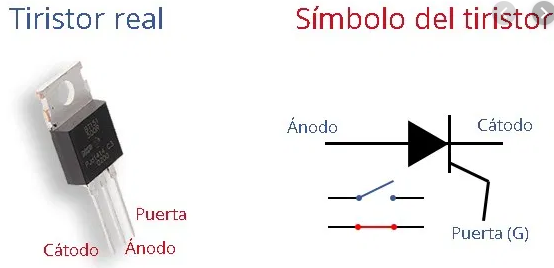
\includegraphics[scale=0.7]{Circuitos/Tiristor.png}
\caption{Tiristor}
\end{figure}

\section*{Tiristores GTO}
Presenta la ventaja de que se puede apagar mediante un impulso de corriente negativo en su puerta. Su principal inconveniente está en las elevadas pérdidas de conmutación, ya que el impulso que se ha de proporcionar para su apagado tiene una amplitud cinco veces menor, aproximadamente, que la corriente a bloquear. Pero el contrario sus pérdidas en conducción son reducidas.\\
Es capaz de manejar grandes tensiones y corrientes (hasta 4,500V y 3,000A).Su aplicación está limitada a convertidores de frecuencia de elevada potencia con circuito intermedio de tensión.
\begin{figure}[hbtp]
\centering
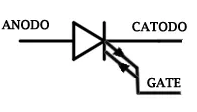
\includegraphics[scale=0.7]{Circuitos/TiristorGTO.png}
\caption{Tiristor GTO}
\end{figure}

\newpage
\section*{Tiristor IGCT}
Los tiristores controlados de puerta aislada (IGCT's)combinan las cualidades de los tiristores (como la baja resistencia en conducción, o su robustez) con la de los IGBT's (capacidad de apagado por puerta o los niveles de corriente de saturación).\\
Por ejemplo las pérdidas de potencia por conmutación de un IGCT son entre y cuatro veces (depende de la tensión de trabajo) menores que las de un IGBT, mientras que la caída de tensión en conducción es la misma.
\begin{figure}[hbtp]
\centering
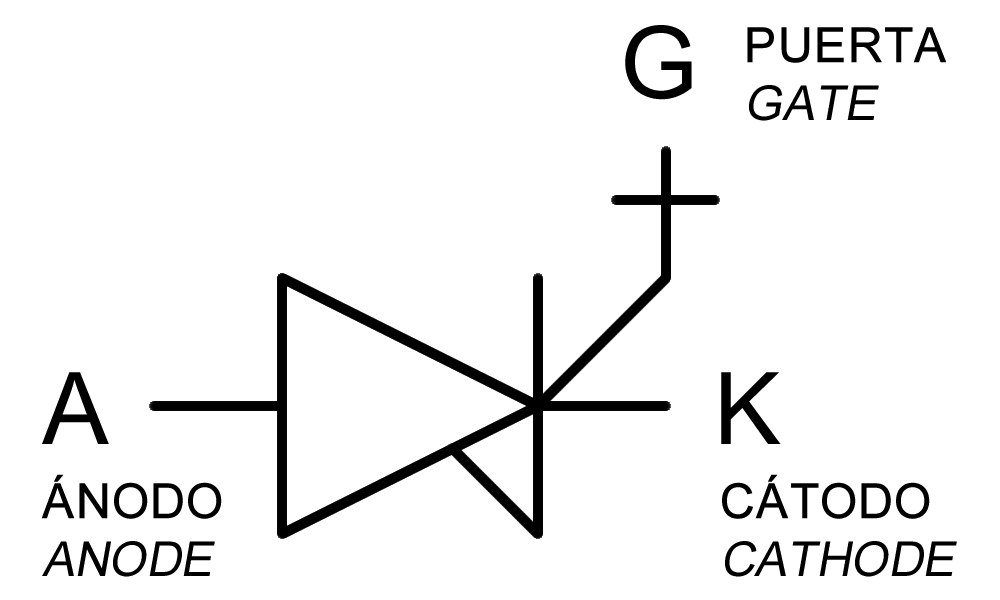
\includegraphics[scale=0.2]{Circuitos/TiristorIGCT.png}
\caption{Tiristor IGCT}
\end{figure}

\section{Convertidor CA-CD}
\subsection{Controlados}
Se puede regular la magnitud de la tensión CC mediante el control de la zona de conducción de los semiconductores de cada fase.\\ 
Tradicionalmente se construyen con tiristores de los que se controla el instante de comienzo de conducción (control por fase). La extinción se produce de forma natural: cuando pasa la corriente por cero o cuando se dispara el tiristor de otra fase hacia el que se desvía la corriente continua.

\begin{figure}[hbtp]
\centering
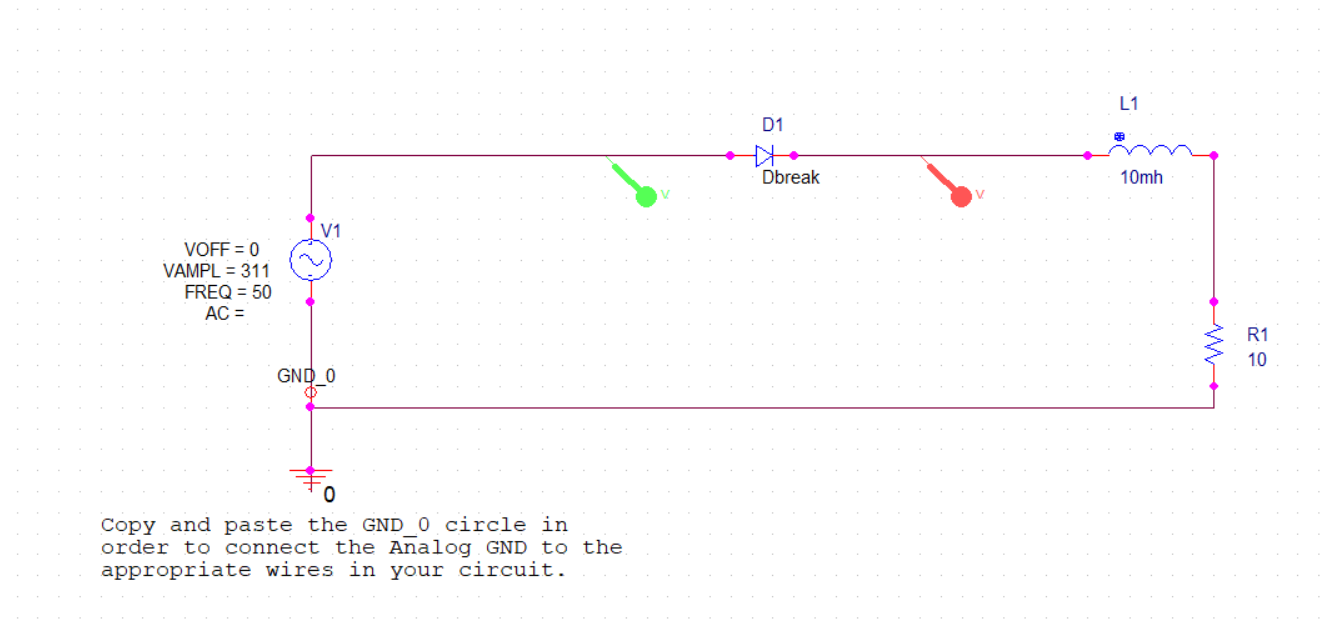
\includegraphics[scale=1]{Circuitos/1.png}
\caption{Rectificador controlado de media onda}
\end{figure}
El disparo de los tiristores se retrasa un ángulo 'a' respecto al cruce de las fases.\\
El funcionamiento depende de y del carácter de la carga. 
\newpage
\begin{figure}[hbtp]
\centering
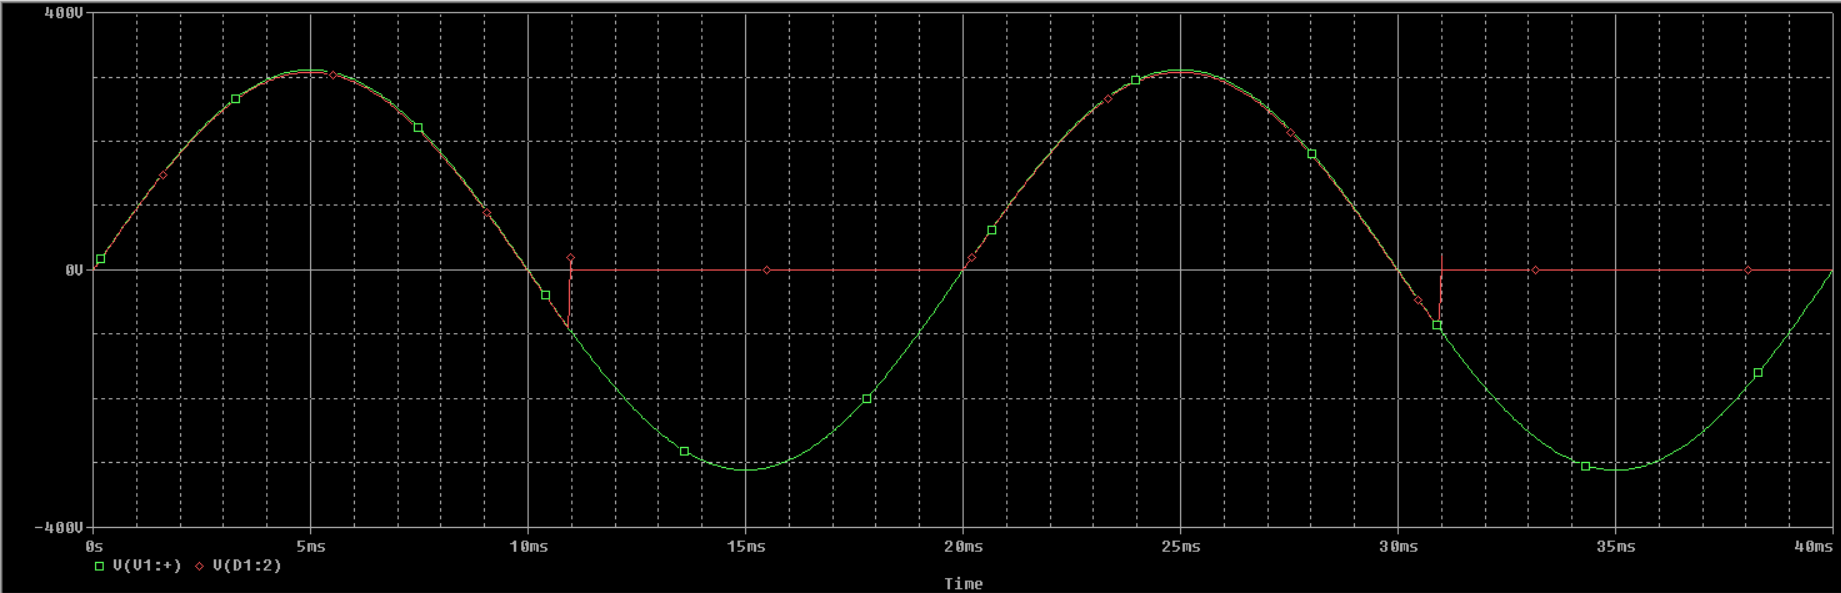
\includegraphics[scale=1]{Circuitos/2.png}
\caption{Rectificador controlado de media onda}
\end{figure}
Observamos el ángulo formado por las tres señales senoidales. 

\section*{Puente controlado}
\begin{figure}[hbtp]
\centering
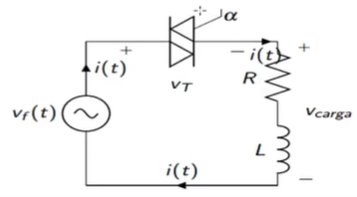
\includegraphics[scale=1]{Circuitos/1_1.png}
\caption{Puente controlado}
\end{figure}
Tenemos dos tiristores en antiparalelo y tenemos control de ambos semiciclos, la forma de la onda será simétrica ambos semiciclos serán iguales lo que conlleva que el valor medio de la onda generada sobre la carga tenga valor -=0.

\newpage
\subsection{Semicontrolados}
Se construyen de forma mixta con diodos y tiristores y pueden controlar la magnitud de la tensión continua de salida, aunque de manera menos flexible.\\

\begin{figure}[hbtp]
\centering
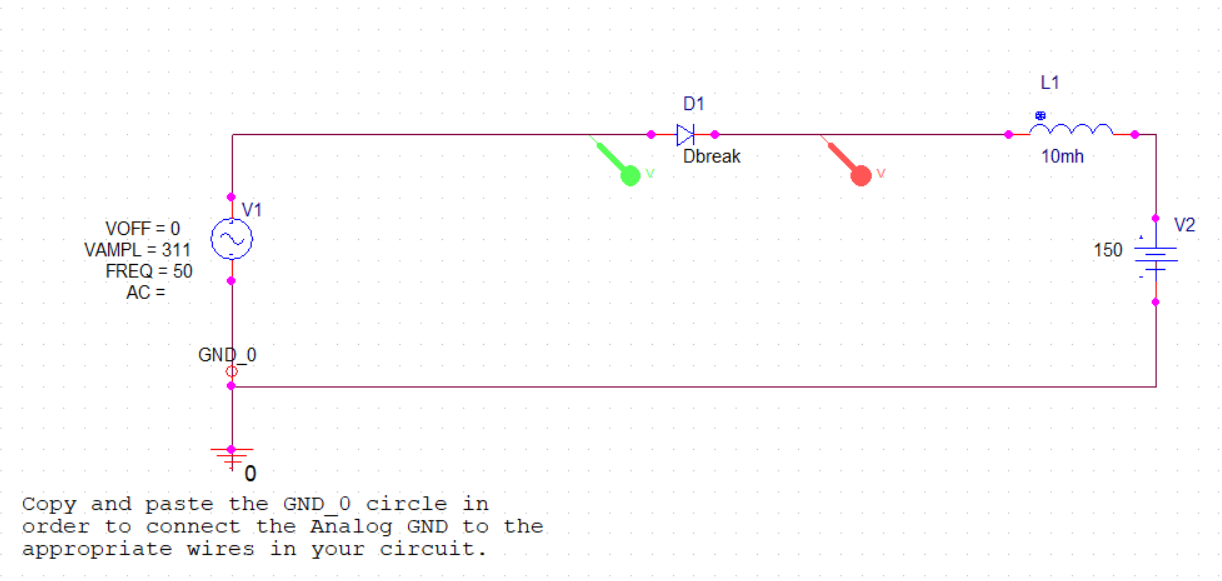
\includegraphics[scale=0.7]{Circuitos/3.png}
\caption{Circuito Semicontrolado}
\end{figure}
Está conformado con un tiristor y por un diodo.El tiristor permite controlar el semiciclo positivo de la carga mientras que el diodo se encargará de pasar el semiciclo negativo de la carga.

\section{Convertidor CA-CA}
\subsection{Ciclo convertidores}
Basan su funcionamiento en el uso de los rectificadores controlados, en donde se cambia la consigna de control con la finalidad de utilizar la misma topología de puente convertidor en otra aplicación. 

\begin{figure}[hbtp]
\centering
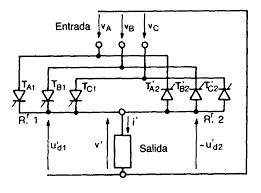
\includegraphics[scale=0.7]{Circuitos/4.png}
\caption{Circuito ciclo convertidor}
\end{figure} 
La tensión de salida hacia la barra de corriente continua puede se positiva o negativa en función de valor de alpha (a), con corriente siempre positiva. 
Permiten realizar una conversión directa CA-CA tanto en la amplitud como en frecuencia sin paso intermedio por CC.\\
Tiene funcionamiento en cuatro cuadrantes: puede funcionar tanto en cargas pasivas como en cargas regenerativas y para cualquier factor de potencia. La frecuencia de salida es menor o igual que la frecuencia de entrada. 

\newpage
\begin{figure}[hbtp]
\centering
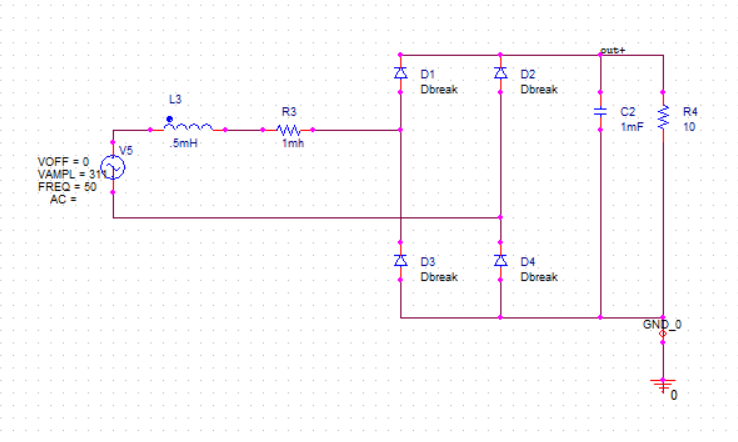
\includegraphics[scale=1]{Circuitos/5.png}
\caption{Salida de tensión}
\end{figure}
Observamos las salidas de tensión de las 3 fases línea a línea b-a-b,b-b-c,b-c-a en caso continuo y en caso discontinuo o punteado los complementos.\\
En Línea gris. Tensión en la barra de corriente continua, correspondiente a un ángulo indeterminado.
La variación del ángulo de encendido es más lenta comparada con la frecuencia de la tensión de entrada w y define la frecuencia de la onda de salida w out.Esto origina que la tensión media sobre la barra de corriente continua varié en cada periodo de la onda de salida en función de la variación del ángulo de encendido 'alpha'.

\section*{Referencias bibliográficas}
Youtube.\\
\url{https://www.youtube.com/watch?v=R7CCiq06HH8}\\
\url{https://www.youtube.com/watch?v=WEhvzgpTbWM}\\
 Basadas en presentaciones.\\
\url{https://slideplayer.es/slide/322441/}
 
\end{document}